%; whizzy chapter
% -initex iniptex -latex platex -format platex -bibtex jbibtex -fmt fmt
% 以上 whizzytex を使用する場合の設定。

%     Kansai Debian Meeting resources
%     Copyright (C) 2007 Takaya Yamashita
%     Thank you for Tokyo Debian Meeting resources

%     This program is free software; you can redistribute it and/or modify
%     it under the terms of the GNU General Public License as published by
%     the Free Software Foundation; either version 2 of the License, or
%     (at your option) any later version.

%     This program is distributed in the hope that it will be useful,
%     but WITHOUT ANY WARRANTY; without even the implied warranty of
%     MERCHANTABILITY or FITNESS FOR A PARTICULAR PURPOSE.  See the
%     GNU General Public License for more details.

%     You should have received a copy of the GNU General Public License
%     along with this program; if not, write to the Free Software
%     Foundation, Inc., 51 Franklin St, Fifth Floor, Boston, MA  02110-1301 USA

%  preview (shell-command (concat "evince " (replace-regexp-in-string "tex$" "pdf"(buffer-file-name)) "&"))
% 画像ファイルを処理するためにはebbを利用してboundingboxを作成。
%(shell-command "cd image200708; ebb *.png")

%%ここからヘッダ開始。

\documentclass[mingoth,a4paper]{jsarticle}
\usepackage{kansaimonthlyreport}
\usepackage[dvips]{xy}
\usepackage{ulem}

% 日付を定義する、毎月変わります。
\newcommand{\debmtgyear}{2013}
\newcommand{\debmtgdate}{24}
\newcommand{\debmtgmonth}{3}
\newcommand{\debmtgnumber}{70}

\begin{document}

\begin{titlepage}

% 毎月変更する部分、本文の末尾も修正することをわすれずに

 第\debmtgnumber{}回 関西 Debian 勉強会資料

\vspace{2cm}

\begin{center}
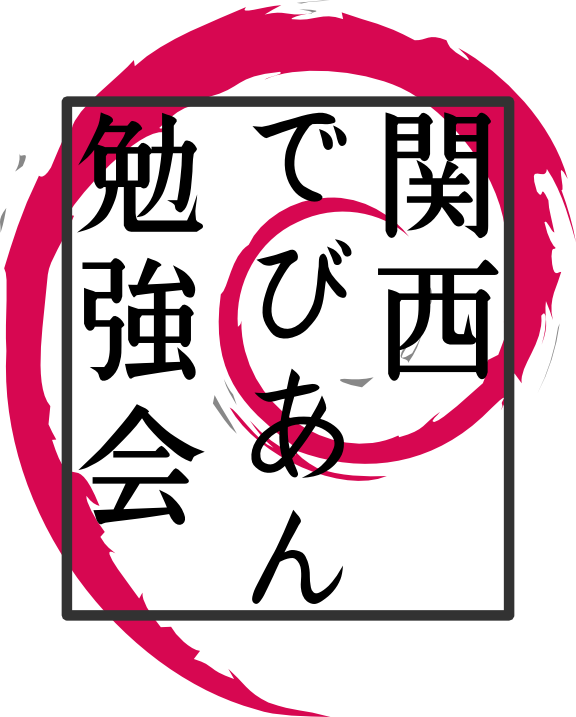
\includegraphics{image200802/kansaidebianlogo.png}
\end{center}

\begin{flushright}
\hfill{}関西 Debian 勉強会担当者 佐々木・倉敷・のがた・かわだ・八津尾 \\
\hfill{}\debmtgyear{}年\debmtgmonth{}月\debmtgdate{}日
\end{flushright}

\thispagestyle{empty}
\end{titlepage}

\dancersection{Introduction}{Debian JP}

\vspace{1em}

 関西Debian勉強会はDebian GNU/Linuxのさまざまなトピック
 (新しいパッケージ、Debian特有の機能の仕組、Debian界隈で起こった出来事、
 などなど)について話し合う会です。

 目的として次の三つを考えています。
 \begin{itemize}
  \item MLや掲示板ではなく、直接顔を合わせる事での情報交換の促進
  \item 定期的に集まれる場所
  \item 資料の作成
 \end{itemize}

 それでは、楽しい一時をお楽しみ下さい。

\newpage

\begin{minipage}[b]{0.2\hsize}
 {\rotatebox{90}{\fontsize{80}{80}
{\gt 関西 Debian 勉強会}}}
\end{minipage}
\begin{minipage}[b]{0.8\hsize}
\hrule
\vspace{2mm}
\hrule
\setcounter{tocdepth}{1}
\tableofcontents
\vspace{2mm}
\hrule
\end{minipage}

\dancersection{最近のDebian関係のイベント報告}{Debian JP}

\subsection{第 69 回関西 Debian 勉強会}

69 回目の関西 Debian 勉強会は 2 月 24 日(日)に GREE さんの
大阪オフィスセミナールームをお借りして行なわれました。

Yuryu さんの「Debian Installer トラブルシューティング」は preseed を使ったインストール
の自動化の実践的内容でした。

佐々木さんの「Ruby In Wheezy」は、みなさんが頭を悩ます Gem や Ruby の複数の実装と
つきあっていくためのヒントが満載でした。

どちらのセッションも参考になった方が多いのではないでしょうか。

GREE 大阪オフィスセミナールームは設備も充実しており綺麗な会場でした。
電話会議システムを使ったプレゼンなど、新しい試みをすることもできました。
今後も機会があればぜひお借りしたいですね。

\subsection{関西 Debian 勉強会 2013 OSC 徳島出展}

3 月 9 日(土) に実施されたオープンソースカンファレンス 2013 Tokushima 
に関西 Debian 勉強会 + 姫路 IT 系勉強会として出展し、関西 Debian 勉強会からは
RaspberryPi と MK802 の実機展示をしました。

\subsection{第 98 回東京エリア Debian 勉強会 2013 年 3 月 勉強会}
3 月 16 日(土) にミラクルリナックス株式会社さんの会議室をお借りして、東京エリア 
Debian 勉強会が開催されました。
まえださんによる 「ldapvi \& python-ldap で stress-free life」、
よしださんによる 「月刊 Debhelper」、
野島さんによる 「gdb の python 拡張」、
の発表が行われました。

\dancersection{事前課題}{Debian JP}

今回は以下の課題を出題しました.
\begin{screen}
  \begin{enumerate}
  \item GNOME3 にどんな拡張機能があれば便利か、考えてみて、教えてください。
  \item wheezy(sid) で GNOME3 環境を用意してきてください。
  \item 「Large deployment of GNOME from the administrator's perspective」
    を読んで気になる点、わからない点を教えてください。
    \url{http://fr2012.mini.debconf.org/slides/LargeGnomeDeployment.pdf}
  \end{enumerate}
\end{screen}

参加者の皆さんの解答は以下の通りです。

\begin{prework}{kazuhito\_m}
  \begin{enumerate}
  \item Gnomeというか、Nautilsに対してかもしれませんが…
        ディレクトリ表示ペインの上か下に「CurrentDirでコマンド打てる入力粋」がほしいなと。すでにあるのでしょうか?
  \item 一応入れてきました。しかし…仮想機だからか「GnomeShellっぽいやつ」が全滅しています。
        世のスクショの画面と同じにならない…一応「GnomeClassic」じゃなく「Gnome」にはなって居るのですが…。 
  \item すみません、読み中です。(会場であればお話を)
  \end{enumerate}
\end{prework}

\begin{prework}{yyatsuo}
  \begin{enumerate}
  \item  (できるのかもしれませんが…) キーボードで window を操作したい 
  \item 用意しました。が、ログインマネージャは slim です
  \item わからないことだらけだったので皆様に教えていただきたく。
  \end{enumerate}
\end{prework}

\begin{prework}{山下尊也}
  \begin{enumerate}
  \item
  \begin{itemize}
    \item shellshape
    \item Remove User Name
    \item TaskBar
    \item Advanced Settings in UserMenu
    \item Alternative Status Menu
    \item Axe Menu
    \item User Themes
    \item Impatience
    \item Frippery Move Clock
  \end{itemize}
  すでに拡張機能入れすぎて、自分が何で満足しているのか分からなくなっているという...
  タイル型の拡張で良いのがあれば良いですね。
  まぁ面倒なんで、いつも最大表示にしちゃいますけど。
  後、タスクバーのアイテムが動かせないのも許せなかったです。
  なんで、時間が真ん中なの!!とか最初思ったので。
  \item これはインストール済み。
  \item 特になしです。というか、まだ読めてない...orz 
  \end{enumerate}
\end{prework}

\begin{prework}{山城の国の住人 久保博 }
  \begin{enumerate}
  \item 時間毎のタイプ頻度とかマウスの移動距離とかをグラフ化する。何時頃に何をしていたか思い出すヒントに。
  \item はい、 wheezy の GNOME3 環境を用意します。
  \item これから何とか
  \end{enumerate}
\end{prework}

\begin{prework}{よしだともひろ}
  \begin{enumerate}
  \item 思いつきませんでした。
  \item 入っています。
  \item すみません、当日読むことになりそう。
  \end{enumerate}
\end{prework}

\begin{prework}{ikuya}
  \begin{enumerate}
  \item 質問者なのでパスで。。
  \item 用意しました。持っていきます。
  \item 21ページ目のNTPはNFSの間違いではないでしょうか?
  \end{enumerate}
\end{prework}

\begin{prework}{lurdan}
  \begin{enumerate}
  \item 余分な装飾と常駐プロセスをまとめて無効化できる的な何か、あるいはタイル(ry
  \item ゴメンね?
  \item 特には。参考になる+1 という感じです。
  \end{enumerate}
\end{prework}


\begin{prework}{水野源}
  無回答
\end{prework}

\begin{prework}{かわだてつたろう}
  \begin{enumerate}
  \item マウスジェスチャー。
  \item はい。
  \item 設定の具体例がもっと欲しい。
  設定を変更するにはどこをさわればよいかは理解したけれど、設定を変更するとどういうことが出来るようになるかまでは理解できていない。
Jessie で変わるところ(systemd、JavaScript での設定)も気になります。
  \end{enumerate}
\end{prework}

\begin{prework}{0xBCD1BC92}
  \begin{enumerate}
  \item Gnome Calendar と Google Calendar の同期
  \item はい
  \item (a) Configuring system connections の Internal と External の前提条件がよくわかりません。例示の具体的なネットワーク図があるとわかりやすいのでは?
        (b) PolicyKit の説明が、ConsoleKitと一緒なので、もうちょい増補してほしいなあ。 
  \end{enumerate}
\end{prework}

\begin{prework}{mkamotsu}
  \begin{enumerate}
  \item 無回答
  \item 無回答
  \item gnome-keyringの仕組みを全く理解してませんでしたが、上記資料のおかげでGNOME環境でなくても利用する方法がわかりました。
(Debian-specific)の部分はアップストリームでどうなっているのか、またどういった理由で手を加えているのかが気になります。
  \end{enumerate}
\end{prework}

\begin{prework}{佐々木洋平}
  とりあえず。課題はあとで。
\end{prework}

\dancersection{Ubuntu と GNOME Shell と私}{あわしろいくや}

\vspace{1em}

\subsection{GNOME Shell の使い方を手っ取り早く知るのに便利な Web ページ}
\begin{itemize}
  \item GnomeShell/CheatSheet
  \item \url{https://live.gnome.org/GnomeShell/CheatSheet}
  \item 若干古いものの、絶大に役に立つ
\end{itemize}

\subsection{筆者の執筆による GNOME Shell 関連記事}
\subsubsection{Ubuntu Weekly Recipe}
\begin{itemize}
  \item \url{http://gihyo.jp/admin/serial/01/ubuntu-recipe/0197}
  \item \url{http://gihyo.jp/admin/serial/01/ubuntu-recipe/0203}
  \item \url{http://gihyo.jp/admin/serial/01/ubuntu-recipe/0219}
  \item \url{http://gihyo.jp/admin/serial/01/ubuntu-recipe/0254}
  \item \url{http://gihyo.jp/admin/serial/01/ubuntu-recipe/0258}
\end{itemize}

\subsubsection{アスキードットテクノロジーズ 2011 年 8 月号}
\begin{itemize}
  \item Fedora15 に見る最新 Linux
  \item 入手困難
\end{itemize}

\subsubsection{Ubuntu Magazine Japan vol.10}
\begin{itemize}
  \item GNOME Remix で快適デスクトップ
  \item 好評発売中
\end{itemize}

\subsection{GNOME Shell のいいところ}
\begin{itemize}
  \item アプリケーションの分類が GNOME 2.x 系列と同じ
  \begin{itemize}
    \item 3.6 まで
  \end{itemize}

  \item 任意に増減できるワークスペース
  \begin{itemize}
    \item 役割は好きに設定
    \item Ctrl+Alt+↑↓
  \end{itemize}

  \item Dash to Dock の存在
  \begin{itemize}
    \item \url{https://extensions.gnome.org/extension/307/dash-to-dock/}
    \item Dash を Dock にできる
    \item Dash...左端に出るラウンチャー
    \item Dock...拡張機能。右端に表示される。普段は隠れている
  \end{itemize}

  \item 豊富な拡張機能
  \begin{itemize}
    \item \url{http://extensions.gnome.org/}
    \item 皆さんが欲しい拡張機能は?
  \end{itemize}

  \item UI があまり変わらない
  \begin{itemize}
    \item ただし 3.0 〜 3.4 まで……
  \end{itemize}
\end{itemize}

\subsection{Ubuntu と GNOME}
\begin{itemize}
  \item Ubuntu 11.10...GNOME 3.2
  \item Ubuntu 12.04...GNOME 3.4
  \begin{itemize}
    \item Wheezy も 3.4
  \end{itemize}
  \item Ubuntu 12.10...GNOME 3.6
  \begin{itemize}
    \item Ubuntu GNOME Remix リリース
  \end{itemize}
  \item Ubuntu 13.04...GNOME 3.6
  \begin{itemize}
    \item Ubuntu GNOME リリース
    \item Unity は GNOME fallback に依存してたが、3.8 からなくなることになった
    \item 開発サイクルの中で GNOME fallback 依存をやめられるかが不透明だったので 3.8 を見送った
  \end{itemize}
\end{itemize}

\subsection{GNOME と IBus}
\subsubsection{GNOME 3.6でIBus 1.5を統合}
\subsubsection{IBus も "GNOME 化"}
\begin{itemize}
  \item 機能の削除
  \begin{itemize}
    \item ツールバーがなくなった
    \item 「すべてのアプリケーション間で同じインプットメソッドを共有する」強制
    \item IBus 1.4.x のアイコンが表示されなくなった
    \begin{itemize}
      \item (Ubuntu の場合) Appindicator Support 拡張をインストール
      \item \url{https://extensions.gnome.org/extension/615/appindicator-support/}
    \end{itemize}
  \end{itemize}
\end{itemize}

\clearpage

\dancersection{Large Deployment of GNOME from the Administrator's Perspective}{八津尾}

Mini Debconf Paris 2012 で発表された Josselin Mouette さんによる 「Large deployment of GNOME from the administrator's perspective」
を読んでみましょう。

GNOME3 を大量にデプロイするケースについて管理者視点から述べた資料ですが、GNOME3 の内部構造について説明されているためユーザ視点で読んでも参考になる資料です。

原著者による GPLv2 or Later での公開に同意いただけなかったため資料は別途用意します。

\clearpage

% ページ調整用
% \dancersection{月刊 Debian Policy 「オペレーティングシステム」その2}{担当:のがた}
% すみません。今回もお休みです。
% \clearpage

\dancersection{今後の予定}{Debian JP}

\subsection{関西 Debian 勉強会}
次回、第 71 回関西 Debian 勉強会は 4 月 28 日(日)に福島区民センターで行ないます。

セッション内容は未定ですが、新年度入門ネタ、きっとリリースされているであろう Wheezy インストール大会になるんじゃないかと思われます。

\subsection{東京エリア Debian 勉強会}
第 99 回東京エリア Debian 勉強会は会場、内容ともに未定ですが 4 月 20 日(土)に開催される予定です。

\subsection{第03回福岡 Debian 勉強会}
福岡で 3 回目となる勉強会、第03回福岡 Debian 勉強会が今週、3 月 28 日(木)に天神セントラルプレイス OnRamp 内で開催されます。

内容は小室さんによる「Wheezyで搭載されるカーネルの新機能とかとか」などが予定されています。

\subsection{大統一 Debian 勉強会}
昨年の 6 月に京都大学で開催された大統一 Debian 勉強会が今年も開催されることになりました。

今年は 6 月 29 日(土)に東京の日本大学駿河台キャンパスで行なわれます。

詳細はまだ決まっていないようですが、4 月上旬にサイト公開予定となっていますので月が変わったら確認してみてください。\footnote{\url{http://gum.debian.or.jp/}}

今から 6 月 29 日の予定を空けて東京行きのチケットを確保しましょう!


% 冊子にするために、4の倍数にする必要がある。
% そのための調整
%\dancersection{メモ}{}
% \mbox{}\newpage
%% \mbox{}\newpage
%% \mbox{}\newpage

\printindex
%\cleartooddpage

 \begin{minipage}[b]{0.2\hsize}
  \rotatebox{90}{\fontsize{80}{80} {\gt 関西 Debian 勉強会} }
 \end{minipage}
 \begin{minipage}[b]{0.8\hsize}

 \vspace*{15cm}
 \rule{\hsize}{1mm}
 \vspace{2mm}
 
\includegraphics[width=2cm]{image200502/openlogo-nd.eps}
 \noindent \Large \bf Debian 勉強会資料\\ \\
 \noindent \normalfont \debmtgyear{}年\debmtgmonth{}月\debmtgdate{}日 \hspace{5mm}  初版第1刷発行\\
 \noindent \normalfont 関西 Debian 勉強会 (編集・印刷・発行)\\
 \rule{\hsize}{1mm}
 \end{minipage}

\end{document}
